\documentclass{beamer}
\beamertemplatenavigationsymbolsempty

\usecolortheme{beaver}
\setbeamertemplate{blocks}[rounded=true, shadow=true]
\setbeamertemplate{footline}[page number]
\setbeamercolor{itemize item}{fg=red}
\setbeamercolor{enumerate item}{fg=red}

\usepackage[utf8]{inputenc}
\usepackage[english,russian]{babel}
\usepackage{amssymb,amsfonts,amsmath,mathtext, dsfont}
\usepackage{makecell} % diaghead in a table
\usepackage{subfig}
\usepackage{tabularx}
\usepackage{array}
\usepackage{multicol, multirow}
\usepackage{hyperref}
\usepackage{hhline}

\usepackage{tikz}
\usetikzlibrary{matrix}

\newcommand{\bx}{\mathbf{x}}
\newcommand{\by}{\mathbf{y}}
\newcommand{\bz}{\mathbf{z}}
\newcommand{\bw}{\mathbf{w}}
\newcommand{\bY}{\mathbf{Y}}
\newcommand{\bX}{\mathbf{X}}
\newcommand{\dH}{\mathds{H}}

\newcommand{\T}{^{\mathsf{T}}}

\graphicspath{{../figures/}}

\title[\hbox to 56mm{Определение фазы}]{Восстановление траектории \\ движения руки по видео}
\author[Э.\,А. Владимиров]{Владимиров Эдуард Анатольевич}
\institute{Московский физико-технический институт}
\date{\footnotesize
	\par\smallskip\emph{Курс:} Моя первая научная статья
	\par\smallskip\emph{Эксперт:} Р.\,В.~Исаченко
	\par\smallskip\emph{Консультанты:} А.\,Д.~Курдюкова
	\par\bigskip\small 2022}

\def\vec#1{\mathchoice{\mbox{\boldmath$\displaystyle#1$}}
	{\mbox{\boldmath$\textstyle#1$}} {\mbox{\boldmath$\scriptstyle#1$}} {\mbox{\boldmath$\scriptscriptstyle#1$}}}

\begin{document}
	\begin{frame}
		\thispagestyle{empty}
		\maketitle
	\end{frame}

	\begin{frame}{Цель исследования}
		
		\begin{alertblock}{Задача}
			Обобщение методов канонического корреляционного анализа с помощью метода Сугихары.
		\end{alertblock}
		
		\begin{alertblock}{Проблема}
			Получение траекторного пространства по временному ряду и выбор метрики для CCM
		\end{alertblock}
		
		\begin{alertblock}{Решение}
			Построение матрицы сдвигов по временному ряду и обучение представления фазового пространства.
		\end{alertblock}
	\end{frame}

	\begin{frame}[fragile]{Методы понижения размерности и метод Сугихары}
		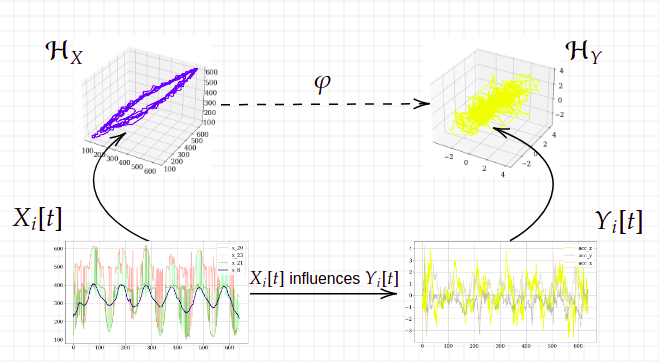
\includegraphics[height=4.5cm]{block_scheme_2.png}
				
		\begin{multicols}{2}
		\begin{tikzpicture}[scale=0.22]
			\matrix (m) [matrix of math nodes,row sep=3em,column sep=4em,minimum width=2em]
			{
				\underset{n \times d}{\bX} & \underset{n \times t}{\bY} \\
				\underset{n \times K}{\mathbf{T}} & \underset{n \times K}{\mathbf{U}} \\};
			\path[-stealth]
			(m-2-1) edge node [right] {$P^T$} (m-1-1)
			(m-2-2) edge node [left] {$Q^T$} (m-1-2)
			(m-1-1) edge [bend right] node [left] {$A$} (m-2-1)
			(m-1-2) edge [bend left] node [right] {$B$} (m-2-2)
			(m-2-1) edge [<->] node [above] {$cov/corr$} (m-2-2)
			(m-1-1) edge [->] node [above] {$f$} (m-1-2);
		\end{tikzpicture}
		\hspace{2cm}
		$T = XA, \: X = T P^T$
		$U = YB, \: Y = U Q^T$
		\hspace{2cm}
		\par
		$\varphi: \bx_{t_0} \mapsto \widehat{\by_{t_0}} = \sum\limits_{i=1}^k w_i \by_{t_i}$
		\end{multicols}
	\end{frame}

	\begin{frame}{Статьи по теме}
		\begin{enumerate}
			\item Edward De Brouwer, Adam Arany, Jaak Simm, and Yves Moreau. Latent convergent
			cross mapping. In International Conference on Learning Representations, 2020
			\item Ricky TQ Chen, Yulia Rubanova, Jesse Bettencourt, and David K Duvenaud. Neural
			ordinary differential equations. Advances in neural information processing systems, 31,
			2018
			\item Farukh Yur’evich Yaushev, Roman Vladimirovich Isachenko, and Vadim Strijov.
			Concordant models for latent space projections in forecasting. Sistemy i Sredstva
			Informatiki [Systems and Means of Informatics], 31(1):4–16, 2021.
		\end{enumerate}
	\end{frame}

	\begin{frame}{Метод Сугихары}
		\begin{itemize}
			\item[\textbullet] Траекторная матрица
			\[ \textbf{H}_{\bx} = \begin{bmatrix}
				x_1 & x_2 & \ldots & x_{n-N+1} \\
				x_2 & x_3 & \ldots & x_{n-N+2} \\
				\vdots & \vdots & \ddots & \vdots \\
				x_{N} & x_{N+1} & \ldots & x_n
			\end{bmatrix}\]
		
			\item[\textbullet] Определение отображения $\varphi$ между траекторными пространствами
			\[ \varphi: \bx_0 \mapsto \widehat{\bz_0} = \sum\limits_{i=1}^k w_i \bz_{t_i}, \quad 
			w_i = \dfrac{u_i}{\sum\limits_{j=1}^k u_j}, \quad
			u_i = \exp(-||\bx_0 - \bx_{t_i}||). \]
			
			\item[\textbullet] Связанные временные ряды
			\[ \rho_{\dH_{\bz}}(\phi(\bx_i), \phi(\bx_j)) \leq C \rho_{\dH_{\bx}}(\bx_i, \bx_j) \qquad \bx_i, \bx_j \in \dH_{\bx} \]
			
			\item[\textbullet] Метрика связанности временных рядов
			\[ Score_{X \rightarrow Z} = CCM_{full}(X, Z) - CCM_0(X, Z) \]
		\end{itemize}
	\end{frame}

	\begin{frame}{Предсказательная модель SMap}
		\begin{itemize}
			\item[\textbullet] Пусть задана обучающая выборка
			\[ \mathfrak{D} = \{ (\bx_i, y_i) \: | \: i = 1, \ldots, d \} = (\bX, \by).\]
			
			\item[\textbullet] В одномерном случае:
			\[ \bx_i = [x_i, x_{i+1}, \ldots, x_{i+N-1}]\T, \quad y_i = x_{i+N}. \]
			
			\item[\textbullet] Каждому $\bx_i \in X \backslash \{ x_{t_0}\}$ сопоставим: \[ \bw_i = \exp \left(-\dfrac{\theta \cdot ||\bx_i - \bx_{t_0}||}{\dfrac{1}{d-1} \sum\limits_{j=1, j \neq t_0}^d ||\bx_j - \bx_{t_0}||} \right). \]
			
			\item[\textbullet] Для прогнозирования используется авторегрессионная модель порядка $t_0-1$:
			\[ X_{t_0} = \mu + \psi_1 X_{t_0-1} + \ldots + \psi_{t_0-1} X_1 + u_{t_0}, \quad u_t \sim \mathcal{N}(0, \sigma^2), \quad \psi_p \neq 0.\]
		\end{itemize}
	\end{frame}

	\begin{frame}{Вычислительный эксперимент}
		\begin{alertblock}{Цель}
			Сравнение различных стратегий снижения размерности целевого пространства.
		\end{alertblock}
		
		
		\begin{multicols}{2}
		\begin{figure}
			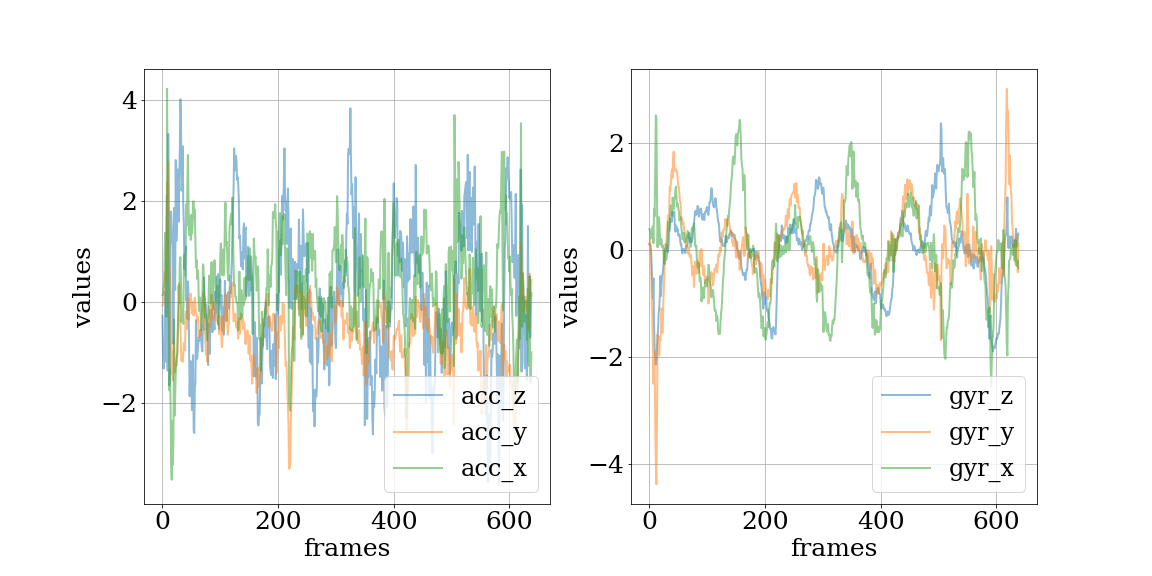
\includegraphics[width=0.5\textwidth]{cyclic_devices_data.png}
			\caption{Данные приборов}
		\end{figure}
	
		\begin{figure}[bhtp]
			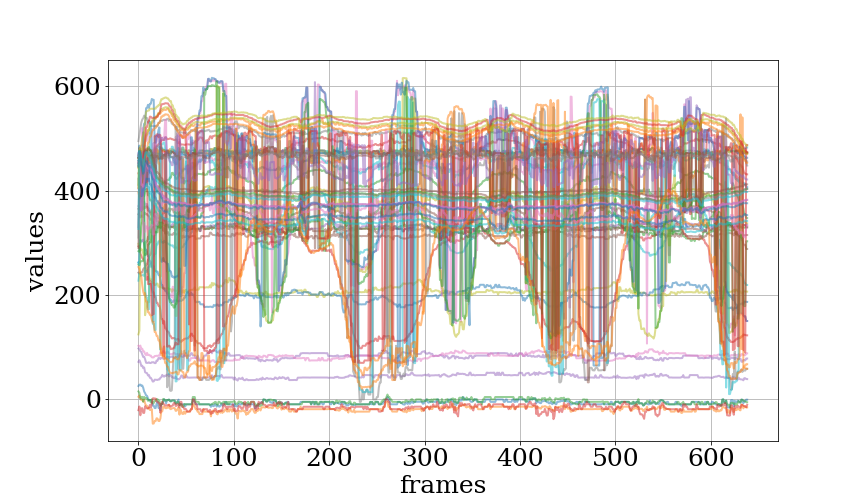
\includegraphics[width=0.5\textwidth]{cyclic_video_data.png}
			\caption{Данные видео-кейпоинтов}
		\end{figure}
		\end{multicols}
		
	\end{frame}

	\begin{frame}{Результаты}
		\begin{table}[bhtp]
			\fontsize{4pt}{8pt}
			\selectfont
			\centering
			\caption{Сравнение ошибки предсказательной модели в траекторном пространстве и в его подпространстве}
			\label{tbl:space_and_subspace}
			\begin{tabularx}{\textwidth}{c|XXXXXX}
				\hline
				& acc\_z & acc\_y & acc\_x & gyr\_z & gyr\_y & gyr\_x \\
				\hline
				space & 1.053 $\pm$ 2.223 & 0.401 $\pm$ 0.833 & 0.483 $\pm$ 0.825 & 0.084 $\pm$ 0.537 & 0.090 $\pm$ 0.094 & 0.063 $\pm$ 0.295 \\
				subspace & 0.315 $\pm$ 0.461 & 0.043 $\pm$ 0.051 & 0.150 $\pm$ 0.177 & 0.001 $\pm$ 0.001	& 0.015 $\pm$ 0.031 & 0.001 $\pm$ 0.003 \\
				\hline
			\end{tabularx}
		\end{table}
	
		\begin{table}[bhtp]
			\tiny
			\centering
			\caption{Сравнение различных методов снижения размерности}
			\label{tbl:methods}
			\begin{tabular}{l|c|llll}
				\hline
				\multicolumn{2}{l}{\diaghead{\hskip4cm}{Целевой признак}{Метод}} \vline & CCM & PLS & CCA & Naive \\
				\hline
				\multirow{6}{*}{\rotatebox[origin=c]{90}{cyclic}} & acc\_z & 0.163 & \textbf{0.040} & 0.116 & 0.141 \\
				& acc\_y & 0.009 & \textbf{0.007} & 0.011 & 0.008 \\
				& acc\_x & \textbf{0.044} & 0.045 & 0.089 & 0.049 \\
				& gyr\_z & \textbf{0.000} & 0.001 & 0.001 & 0.001 \\
				& gyr\_y & \textbf{0.002} & 0.004 & 0.005 & 0.003 \\
				& gyr\_x & 0.009 & 0.004 & 0.004 & \textbf{0.003} \\
				\hline
				\multirow{6}{*}{\rotatebox[origin=c]{90}{chaotic}} & acc\_z & \textbf{0.315} & 0.416 & 0.416 & 0.331 \\
				& acc\_y & \textbf{0.043} & 0.045 & 0.429 & 0.055 \\
				& acc\_x & 0.150 & 0.177 & 0.221 & \textbf{0.143} \\
				& gyr\_z & \textbf{0.001} & 0.002 & 0.003 & 0.003 \\
				& gyr\_y & \textbf{0.015} & 0.022 & 0.061 & 0.026 \\
				& gyr\_x & \textbf{0.001} & 0.013 & 0.015 & 0.008 \\
				\hline   
			\end{tabular}
		\end{table}
	\end{frame}

	\begin{frame}{Заключение}
		\begin{itemize}
			\item[\textbullet] Предложен метод обобщения PLS и CCA с помощью метода Сугихары
			
			\item[\textbullet] Проведён вычислительный эксперимент на данных устройств и видеоряда
			
			\item[\textbullet] Получено, что использование данных из видео повышает качество прогнозирования
			
			\item[\textbullet] Показано, что прогностическая модель менее устойчива в случае, когда та применяется в траекторном пространстве
		\end{itemize}
	\end{frame}

\end{document}
